\section{Case Study: Web eID}

\subsection{About}

Released in the Summer of 2021 \cite{ria-webeid} and having undergone significant changes in January of 2022, this eID framework allows users to authenticate and sign documents using their country's smart cards.

Functionally this framework is split into three parts: software the user needs to install on their computer, a javascript library that acts as a data transfer intermediary, and the certificate validation library for the back-end.

The software users need to install is similar to the one various countries' governments issue. The significant difference is that this software supports more than one countries' eID solutions. Supported countries include Estonia, Latvia, Lithuania, and Finland \cite{ria-webeid}.

This service is built by the Estonian Information System Authority, responsible for TARA, Estonia's public sector gateway. No publicly available audit certification is available at the time of writing \todo{is this true?}.

\subsection{Data Flow}

Figure \ref{fig:web-eid-authentication} displays the high-level overview of the complete flow of data within the Web eID framework. A detailed explanation of the steps can be found on the technical specification page \cite{ria-webeid-systemarchitecture}. Companies implementing the framework should only consider the browser and the server application (steps 1-3 and 13-17).

\begin{figure}
  \centering
  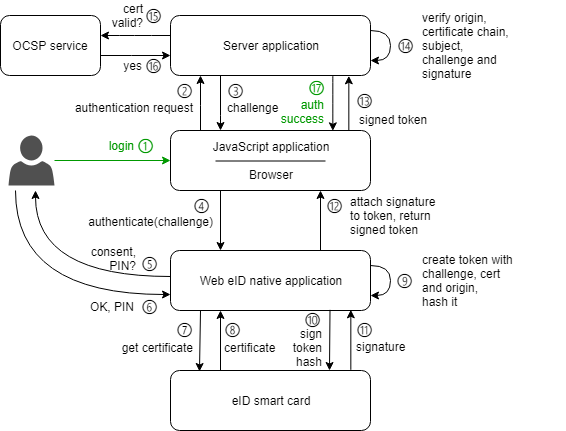
\includegraphics[scale=0.6]{webeid/Web-eID-authentication-communication-diagram}
  \caption{Web eID Authentication flow \cite{ria-webeid-systemarchitecture}}
  \label{fig:web-eid-authentication}
\end{figure}

\TODO{Steps 1-3 ... Steps 13-17}

\subsection{Trust Anchor}

Unlike Dokobit and eeID, Web eID does not provide any guarantees about the trustworthiness of a certificate. It is, however, not out of malice and reminds developers by sending the certificate in a field called "unverifiedCertificate" \cite{ria-webeid-source-web-eid-authtoken-validation-java-readme}.

The relying party must verify the certificate and challenge themselves by checking the origin, certificate expiry, trust chain, OCSP response, and the challenge. This validation structure makes the trust anchor technological and highly dependent on the implementation correctness by the developers.

\subsection{Pricing}

The Web eID authentication service is free of charge, as the only external validation, OCSP \cite{rfc6960} requests, are free to use. When creating digital signatures, the timestamping service may require payment \cite{ria-webeid-source-web-eid-authtoken-validation-java-readme}, however the focus is only on the authentication.

\subsection{Security Requirements}

Web eID is almost entirely an offline protocol; therefore, the IETF guidelines document \cite{ietf-oauth-security-topics-19} used for eeID, and Dokobit is not applicable here. Instead, we will solely rely on the implementation details provided by RIA \cite{ria-webeid-systemarchitecture}.

The second version of the protocol (having accounted for the feedback of Arnis Paršovs \cite{arnis-report-webeid}) will be analyzed.

\paragraph{Communication channel}

The Web eID framework is the only one covered by this thesis that uses an insecure communication channel. Developers must take caution and verify received data when implementing the framework. This channel is highly susceptible to man-in-the-middle, forgery, or other attacks done by the user.

Unlike in the cases of Dokobit and eeID, the risk of impersonation is not transferred to the eID service provider. However, a higher degree of certainty is provided, as only the client can be malicious. The underlying trust anchor, cryptography, is unlikely to be nefarious.

\subsection{Integration}

For each protocol implementation step, developers will have to fulfill certain guarantees before the system goes into production.

\subsubsection{Preparation}

Building the challenge nonce. The goal of these steps is to create the challenge the user will have to sign with their private key. There are a couple of guarantees the application must provide:
\begin{enumerate}
  \item Generated challenge nonce must be between 32 and 96 bytes (inclusive) in length \cite{ria-webeid-source-web-eid-app-authenticate};
  \item "It must be guaranteed that the authentication token is received from the same browser to which the corresponding challenge nonce was issued" \cite{ria-webeid-source-web-eid-authtoken-validation-java-readme}. The framework creators suggest attaching it to the user session.
  \item "Cache must be used for protection against replay attacks by guaranteeing that each authentication token can be used exactly once" \cite{ria-webeid-source-web-eid-authtoken-validation-java-readme}.
  \item "Cookie-based authentication must be protected against cross-site request forgery (CSRF) attacks and extra measures must be taken to secure the cookies by serving them only over HTTPS and setting the HttpOnly, Secure and SameSite attributes" \cite{ria-webeid-source-web-eid-authtoken-validation-java-readme}.
\end{enumerate}

In the implementation example, these measures were addressed by:
\begin{enumerate}
  \item a 64 byte cryptographically secure randomly generated nonce is created (see listing \ref{lst:web-eid-challenge});
  \item challenge nonce is set in the user's session, which adversaries cannot tamper;
  \item the generated nonce is stored into local memory cache for later use; nonce expires after 5 minutes;
  \item an input field is rendered on the page with a unique CSRF validation token, which prevents cross-site request forgery attacks (see listing \ref{lst:web-eid-challenge-ui});
\end{enumerate}

\begin{lstlisting}[caption={Web eID Challenge Endpoint}, label={lst:web-eid-challenge}]
private TimeSpan ChallengeLifetime { get; } = TimeSpan.FromMinutes(5);

private readonly IMemoryCache _cache; // Injected

[HttpGet("challenge")]
public IActionResult GetChallenge()
{
    var nonce = RandomNumberGenerator.GetBytes(64);

    _cache.Set(Convert.ToBase64String(nonce), true, ChallengeLifetime);
    HttpContext.Session.Set("eid.challenge", nonce);

    return Ok(new { nonce });
}
\end{lstlisting}


\begin{lstlisting}[caption={Web eID UI excerpt}, label={lst:web-eid-challenge-ui}, language={html}]
@inject Microsoft.AspNetCore.Antiforgery.IAntiforgery _csrf
@{ var csrfToken = _csrf.GetAndStoreTokens(HttpContext); }

<!-- Button used to sign in -->
<a role="button" class="btn btn-secondary" id="webeid-auth-button">Web eID</a>

<input id="csrfToken" type="hidden" value="@csrfToken.RequestToken"/>

<script>
    ...

    const authTokenResponse = await fetch("/signin-id/login", {
        method: "POST",
        headers: {
            "Content-Type": "application/json",
            "RequestVerificationToken": document.getElementById("csrfToken").value
        },
        body: JSON.stringify(...)
    });

    ...
</script>
\end{lstlisting}

\subsubsection{Validation}

After the user signs the nonce challenge and sends their certificate, the server must verify its authenticity. The application must perform all of the following before allowing the user to sign in:

\begin{enumerate}
  \item verify the CSRF token from earlier steps \cite{ria-webeid-source-web-eid-authtoken-validation-java-readme};
  \item verify the challenge nonce came from the original user and has not expired, was not consumed;
  \item verify the certificate validity and check if nonce was signed by the associated private key (see below);
  \item issue an authentication token with the fields from the certificate's subject;
\end{enumerate}

In the implementation example, these measures were addressed by:
\begin{enumerate}
  \item the back end endpoint for log-in is decorated with ValidateAntiForgeryToken Attribute. This attribute instructs the ASP.NET API to ignore requests not containing a CSRF token \cite{msdocs-anti-request-forgery}. A JavaScript application can only access the protected endpoints by providing RequestVerificationToken header (see listing \ref{lst:web-eid-challenge-ui});
  \item the application tries to extract the challenge nonce from the browsing session. The process would succeed if the session cookie were not modified. After the extraction, the application checks the nonce cache to verify if the challenge is still active. Cache hit means the nonce has not expired, and no previous authentication attempt was performed. Remove the challenge nonce from all stores.
  \item The API calls a standalone validation service to verify the nonce and certificate (see certificate and nonce verification paragraph below).
  \item Application populates the ASP.NET identity management system with the fields from the certificate: serial number, given name, surname, country. An identity session cookie is sent to the client.
\end{enumerate}

\begin{lstlisting}[caption={Web eID Login Endpoint}, label={lst:web-eid-login}]
[HttpPost("login")]
[ValidateAntiForgeryToken]
public async Task<IActionResult> Login([FromBody] WebIdAuthTokenResponse token)
{
    // Obtain the challenge from session
    if (!HttpContext.Session.TryGetValue(ChallengeNonceKey, out var nonce) && nonce == null)
        return Unauthorized();

    // Check if token was not used before or expired
    var challenge = Convert.ToBase64String(nonce);
    if (!_cache.TryGetValue(challenge, out _))
        return Unauthorized();

    _cache.Remove(challenge);
    HttpContext.Session.Remove(ChallengeNonceKey);

    // Validate the certificate and signed challenge
    var validationResult = await _webEidValidationService.GetResult(new WebEidValidationRequest(token, nonce));
    if (!validationResult.Success)
        return Forbid();

    // Certificate is valid. Sign in the user

    await HttpContext.SignInAsync(BuildUser(new X509Certificate2(Convert.FromBase64String(token.UnverifiedCertificate)).Subject));

    return Ok();
}
\end{lstlisting}

\subsubsection{Certificate and nonce verification}

This step is the most complicated in the entire validation process. To prevent any issues with incorrect implementation, the framework maintainers recommend using their library for validation \cite{ria-webeid-source-web-eid-authtoken-validation-java-readme}. Libraries can come with security vulnerabilities, and developers are reluctant to update their used version; however, it is still more favorable to creating vulnerabilities from misconfiguration \cite{9240619}.

The eu.webeid.security Java package performs most of the certificate validation: expiry, purpose, policy, OCSP \cite{ria-webeid-source-web-eid-authtoken-validation-java-readme}. Developers will only have to configure the CA and host validation. Configuration is handled by providing a set of trusted CA certificates for trust chain verification and the hostname for challenge nonces (see listing \ref{lst:web-eid-java-lib}).

\begin{lstlisting}[caption={Web eID Login Endpoint}, label={lst:web-eid-java-lib}]
public class AuthTokenValidatorService {

  @Bean
  public AuthTokenValidator validator() {
    try {
      return new AuthTokenValidatorBuilder()
        .withSiteOrigin(URI.create(System.getenv("ORIGIN_URL")))
        .withTrustedCertificateAuthorities(loadTrustedCACertificatesFromCerFiles())
        .build();
    } catch (JceException e) {
      throw new RuntimeException("Error building the Web eID auth token validator.", e);
    }
  }

  private X509Certificate[] loadTrustedCACertificatesFromCerFiles() {
    List<X509Certificate> caCertificates = new ArrayList<>();

    try {
      CertificateFactory certFactory = CertificateFactory.getInstance("X.509");

      File[] files = new File("/certs").listFiles((f, n) -> n.endsWith(".cer"));
      if (files != null) {
        for (File file : files) {
          try (InputStream stream = new FileInputStream(file)) {
            X509Certificate caCertificate = (X509Certificate) certFactory.generateCertificate(stream);
            caCertificates.add(caCertificate);
          }
        }
      }
    } catch (CertificateException | IOException e) {
      throw new RuntimeException("Error initializing trusted CA certificates.", e);
    }

    return caCertificates.toArray(new X509Certificate[0]);
  }
}
\end{lstlisting}

The token validation service described in listing \ref{lst:web-eid-java-lib} requires WorkAuth maintainers to set the origin URL in the form of an environment variable and to populate the folder {/certs} with trusted CA certificates.

Origin URL can be obtained by checking the {window.origin} JavaScript variable in the page containing the log-in button.

For the CA certificate set, the company can get an up-to-date list of trusted certificates at the EU Trust Services Dashboard \cite{eu-trustservices}. The issue with this list is that it contains all trust certificates for various scopes. In our case, we should limit the search to the extent of QCert for ESig. In the case of Estonia and Lithuania, only three entities are certified to issue certificates for QSCD (see figure \ref{fig:eu-tsp-list}). It is in stark contrast to Spain's 31 \cite{eu-trustservices}. It is possible to further narrow down to only certificate generation services for qualified certificates (CA/QC).

\begin{figure}
  \centering
  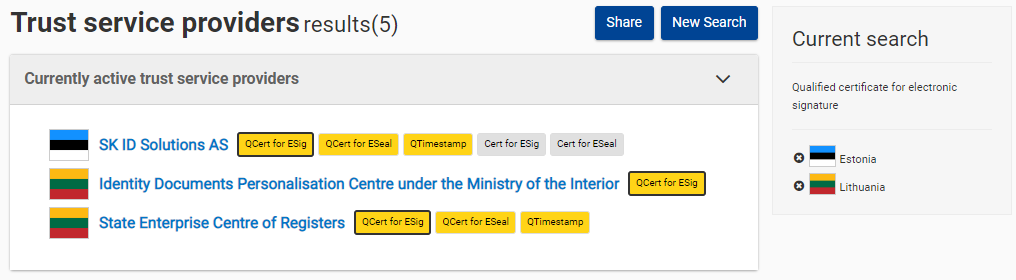
\includegraphics[scale=0.54]{webeid/eu-tsp-search}
  \caption{List of EU Trust service providers of Estonia and Lithuania capable of creating qualified certificates for e-signatures}
  \label{fig:eu-tsp-list}
\end{figure}

In the case of Estonia's single TSP, we can see that only 3 CA are currently operational (see figure \ref{fig:eu-tsp-skid}). Unfortunately, there is no standardized way of narrowing down which certificates could be used for authentication.

\begin{figure}
  \centering
  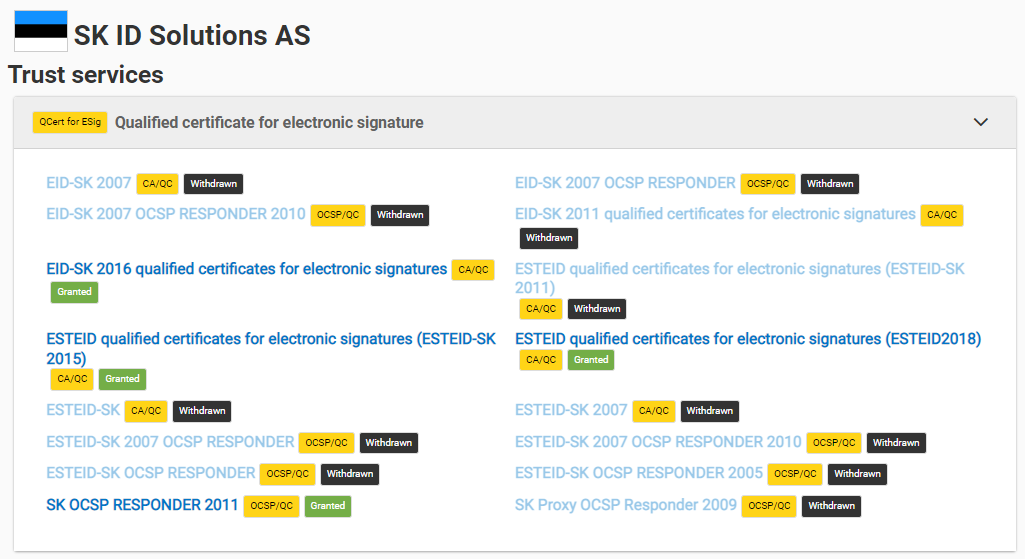
\includegraphics[scale=0.54]{webeid/eu-tsp-skid}
  \caption{List of certificates issued to SK ID Solutions AS for the purposes of Qualified certificate for electronic signature}
  \label{fig:eu-tsp-skid}
\end{figure}

An alternative way to obtain certificates would be to go to the government authority of each country responsible for the distribution of certificates. This action requires prior knowledge of who is responsible for issuing certificates and their purposes.

In Lithuania's case, it is the Ministry of the Interior \cite{eid-lt-ministryofinterior-certificates} who issues two certificates every couple of years. As of early 2022, four certificates are active, and all will be added to the trusted CA list.

In Estonia's case, SK ID Solutions manages the CA certificates \cite{eid-ee-skid-certificates}. Of the three certificates found on the EU Trust Services Dashboard, only two are relevant to us, the 2015 and 2018 ones, as the 2016 one has its purpose for use in Smart-ID, which the Web eID framework does not support.

The final count of certificates is six. Four certificates are required to support Lithuania and two for Estonia. It is essential to keep track of these certificates as each one of them can act as a point of compromise and must be monitored in the event they are revoked for security \cite{roca-vulnerability-lessons-learned} or other issues.

\paragraph{Exposing the service}

With the certificate validation service configured, it is now required to link it to the Web API. If the company orients around using microservices, this service can be just that. All that the validation service requires is to expose an endpoint that accepts a nonce and a token from the javascript library and returns a validation result.

Companies must take proper measures to protect such service from adversaries as it acts as a fundamental trust anchor. Developers should take steps outlined in assume breach \todo{citation missing} to mitigate the risk of misuse with the use of TLS and other countermeasures.
